\documentclass[main.tex]{subfiles}

\begin{document}
\section{Аналитические выводы. Коэффициент прохождения волны}

В этом разделе предполагается, что жёсткости всех пружин в решётках одинаковые.
Масса частиц левой решётки $M_1$; масса частиц правой решётки $M_2$.

Ищем решение уравнений движения в следующем виде (метод трёх волн):
\beq
u_{n,m}=
\begin{cases}
	A_{I}e^{\im\left(\Omega t-ak_1^xn-ak_1^ym\right)}+A_{R}e^{\im\left(\Omega t+ak_1^xn-ak_1^ym\right)},\,\,\,\,\,n<0\\
	A_{T}e^{\im\left(\Omega t-ak_2^xn-ak_2^ym\right)},\,\,\,\,\,n\geqslant 0
\end{cases}
\eeq

Дисперсионное соотношение для решётки:
\beq
M_i\Omega^2=4c\left(\sin^2{\frac{k_i^xa}{2}}+\sin^2{\frac{k_i^ya}{2}}\right)
\eeq


Уравнения движения для частиц интерфейса:
\beq
\begin{cases}
	M_1\ddot{u}_{-1,m}=c\left(u_{0,m}+u_{-1,m+1}+u_{-2,m}+u_{-1,m-1}-4u_{-1,m}\right)\\
	M_2\ddot{u}_{0,m}=c\left(u_{1,m}+u_{0,m+1}+u_{-1,m}+u_{0,m-1}-4u_{0,m}\right)
\end{cases}
\eeq

Получаем:
\beq
\frac{A_T}{A_I}=\frac{e^{\im k_1^xa}-e^{-\im k_1^xa}}{e^{\im k_2^xa}-e^{-\im k_1^xa}}\cdot\frac{e^{\im k_2^y am}}{e^{\im k_1^y am}}
\eeq

\beq
T=\frac{M_2g_2^x}{M_1g_1^x}\left|\frac{e^{\im k_1^xa}-e^{-\im k_1^xa}}{e^{\im k_2^xa}-e^{-\im k_1^xa}}\right|^2,
\eeq
где
$$
g_i=\frac{d\Omega}{dk_i}
$$
\ \newpage
%Из геометрии $k_1^y=k_2^y$.

\section{Поиск производной суммарного потока в решётках}

В этом разделе масса частиц левой решётки $M_1$, жёсткость пружин левой решётки $c_1$; масса частиц правой решётки $M_2$, жёсткость пружин правой решётки $c_2$; жёсткость пружин интерфейса $c_{12}$.

Уравнение движения для частицы $\left(n,m\right)$:
\beq
\label{eqn-motion}
M_{n,m}\dot{v}_{n,m}=F_{n+\frac{1}{2},m}-F_{n-\frac{1}{2},m}+F_{n,m+\frac{1}{2}}-F_{n,m-\frac{1}{2}},
\eeq
где
$$
F_{n+\frac{1}{2},m}=C_{n+\frac{1}{2},m}\varepsilon_{n+\frac{1}{2},m}\hspace{2cm}\varepsilon_{n+\frac{1}{2},m}=u_{n+1,m}-u_{n,m}
$$
$$
F_{n,m+\frac{1}{2}}=C_{n,m+\frac{1}{2}}\varepsilon_{n,m+\frac{1}{2}}\hspace{2cm}\varepsilon_{n,m+\frac{1}{2}}=u_{n,m+1}-u_{n,m}
$$

Выражение для потока:
\beq
\uline{h}_{n+\frac{1}{2},m+\frac{1}{2}}=-\frac{a\uline{e_1}}{2}F_{n+\frac{1}{2},m}\left(v_{n+1,m}+v_{n,m}\right)-\frac{a\uline{e_2}}{2}F_{n,m+\frac{1}{2}}\left(v_{n,m+1}+v_{n,m}\right)
\eeq

Производная потока:
\beq
\label{flux-der}
\begin{aligned}
\uline{\dot{h}}_{n+\frac{1}{2},m+\frac{1}{2}}=
&-\frac{a\uline{e_1}}{2}\dot{F}_{n+\frac{1}{2},m}\left(v_{n+1,m}+v_{n,m}\right)-\\[1ex]
&-\frac{a\uline{e_1}}{2}F_{n+\frac{1}{2},m}\left(\dot{v}_{n+1,m}+\dot{v}_{n,m}\right)-\\[1ex]
&-\frac{a\uline{e_2}}{2}\dot{F}_{n,m+\frac{1}{2}}\left(v_{n,m+1}+v_{n,m}\right)-\\[1ex]
&-\frac{a\uline{e_2}}{2}F_{n,m+\frac{1}{2}}\left(\dot{v}_{n,m+1}+\dot{v}_{n,m}\right).
\end{aligned}
\eeq

Из уравнения движения \eqref{eqn-motion}:
\beq
\label{vels}
\begin{aligned}
\dot{v}_{n,m}&=\frac{F_{n+\frac{1}{2},m}}{M_{n,m}}-\frac{F_{n-\frac{1}{2},m}}{M_{n,m}}+\frac{F_{n,m+\frac{1}{2}}}{M_{n,m}}-\frac{F_{n,m-\frac{1}{2}}}{M_{n,m}}\\[1.5ex]
\dot{v}_{n+1,m}&=\frac{F_{n+\frac{3}{2},m}}{M_{n+1,m}}-\frac{F_{n+\frac{1}{2},m}}{M_{n+1,m}}+\frac{F_{n+1,m+\frac{1}{2}}}{M_{n+1,m}}-\frac{F_{n+1,m-\frac{1}{2}}}{M_{n+1,m}}\\[1.5ex]
\dot{v}_{n,m+1}&=\frac{F_{n+\frac{1}{2},m+1}}{M_{n,m+1}}-\frac{F_{n-\frac{1}{2},m+1}}{M_{n,m+1}}+\frac{F_{n,m+\frac{3}{2}}}{M_{n,m+1}}-\frac{F_{n,m+\frac{1}{2}}}{M_{n,m+1}}
\end{aligned}
\eeq

И знаем, что
\beq
\label{force}
\begin{aligned}
\dot{F}_{n+\frac{1}{2},m}&=C_{n+\frac{1}{2},m}\left(v_{n+1,m}-v_{n,m}\right)\\[1.5ex]
\dot{F}_{n,m+\frac{1}{2}}&=C_{n,m+\frac{1}{2}}\left(v_{n,m+1}-v_{n,m}\right)
\end{aligned}
\eeq

Подставляем \eqref{vels} и \eqref{force} в выражение \eqref{flux-der}:
\beq
\label{flux-der-2}
\begin{aligned}
\uline{\dot{h}}_{n+\frac{1}{2},m+\frac{1}{2}}=&-\frac{a\uline{e_1}}{2}C_{n+\frac{1}{2},m}\left(v_{n+1,m}^2-v_{n,m}^2\right)-\\[1.5ex]
&-\frac{a\uline{e_1}}{2}F_{n+\frac{1}{2},m}\left(\frac{F_{n+\frac{1}{2},m}}{M_{n,m}}-\frac{F_{n+\frac{1}{2},m}}{M_{n+1,m}}+\frac{F_{n+\frac{3}{2},m}}{M_{n+1,m}}-\frac{F_{n-\frac{1}{2},m}}{M_{n,m}}\right.+\\[1.5ex]
&\hspace{3cm}+\left.\frac{F_{n,m+\frac{1}{2}}}{M_{n,m}}-\frac{F_{n,m-\frac{1}{2}}}{M_{n,m}}+\frac{F_{n+1,m+\frac{1}{2}}}{M_{n+1,m}}-\frac{F_{n+1,m-\frac{1}{2}}}{M_{n+1,m}}\right)-\\[1.5ex]
&-\frac{a\uline{e_2}}{2}C_{n,m+\frac{1}{2}}\left(v_{n,m+1}^2-v_{n,m}^2\right)-\\[1.5ex]
&-\frac{a\uline{e_2}}{2}F_{n,m+\frac{1}{2}}\left(\frac{F_{n,m+\frac{1}{2}}}{M_{n,m}}-\frac{F_{n,m+\frac{1}{2}}}{M_{n,m+1}}+\frac{F_{n,m+\frac{3}{2}}}{M_{n,m+1}}-\frac{F_{n,m-\frac{1}{2}}}{M_{n,m}}\right.+\\[1.5ex]
&\hspace{3cm}+\left.\frac{F_{n+\frac{1}{2},m}}{M_{n,m}}-\frac{F_{n-\frac{1}{2},m}}{M_{n,m}}+\frac{F_{n+\frac{1}{2},m+1}}{M_{n,m+1}}-\frac{F_{n-\frac{1}{2},m+1}}{M_{n,m+1}}\right)
\end{aligned}
\eeq

Для неоднородной решётки:
\beq
M_{n,m}=
\begin{cases}
M_1, \hspace{0.5cm} n<0,\\
M_2, \hspace{0.5cm} n\geqslant0,
\end{cases}
\hspace{1cm}
C_{n+\frac{1}{2},m}=
\begin{cases}
c_1, \hspace{0.5cm} n<-1,\\
c_{12}, \hspace{0.5cm} n=-1,\\
c_2, \hspace{0.5cm} n\geqslant0,
\end{cases}
\eeq

Суммируя по всем частицам, получаем:
\beq
\begin{aligned}
\dot{h}=-\frac{a\uline{e_1}}{2}&\left(\sum_{m=-\infty}^{+\infty}{\left[\left(c_{12}-c_2\right)v_{0,m}^2+\left(c_1-c_{12}\right)v_{-1,m}^2\right]}\right.+\\[1.5ex]
&\left.+\sum_{m=-\infty}^{+\infty}{\left(\frac{F_{-\frac{1}{2},m}^2}{M_2}-\frac{F_{-\frac{1}{2},m}^2}{M_1}\right)}\right.+\\[1.5ex]
&\left.+\sum_{m,n}{\left[F_{n+\frac{1}{2},m}\left(\frac{F_{n,m+\frac{1}{2}}}{M_{n,m}}-\frac{F_{n,m-\frac{1}{2}}}{M_{n,m}}+\frac{F_{n+1,m+\frac{1}{2}}}{M_{n+1,m}}-\frac{F_{n+1,m-\frac{1}{2}}}{M_{n+1,m}}\right)\right]}\right)-\\[1.5ex]
&\hspace{-1.1cm}-\frac{a\uline{e_2}}{2}\left(0+0\right.+\\[1.5ex]
&\left.+\sum_{m,n}{\left[F_{n,m+\frac{1}{2}}\left(\frac{F_{n+\frac{1}{2},m}}{M_{n,m}}-\frac{F_{n-\frac{1}{2},m}}{M_{n,m}}+\frac{F_{n+\frac{1}{2},m+1}}{M_{n,m+1}}-\frac{F_{n-\frac{1}{2},m+1}}{M_{n,m+1}}\right)\right]}\right)
\end{aligned}
\eeq

Преобразуем
\beq
\begin{aligned}
\dot{h}=-\frac{a\uline{e_1}}{2}&\left(\sum_{m=-\infty}^{+\infty}{\left[\left(c_{12}-c_2\right)v_{0,m}^2+\left(c_1-c_{12}\right)v_{-1,m}^2\right]}\right.+\\[1.5ex]
&\left.+\sum_{m=-\infty}^{+\infty}{\frac{M_1-M_2}{M_1M_2}}c_{12}^2\varepsilon_{-\frac{1}{2},m}^2\right.+\\[1.5ex]
&\left.+\sum_{m,n}{\left[F_{n+\frac{1}{2},m}\left(\frac{F_{n,m+\frac{1}{2}}}{M_{n,m}}-\frac{F_{n,m-\frac{1}{2}}}{M_{n,m}}+\frac{F_{n+1,m+\frac{1}{2}}}{M_{n+1,m}}-\frac{F_{n+1,m-\frac{1}{2}}}{M_{n+1,m}}\right)\right]}\right)-\\[1.5ex]
&\hspace{-1.1cm}-\frac{a\uline{e_2}}{2}\left(\sum_{m,n}{\left[F_{n,m+\frac{1}{2}}\left(\frac{F_{n+\frac{1}{2},m}}{M_{n,m}}-\frac{F_{n-\frac{1}{2},m}}{M_{n,m}}+\frac{F_{n+\frac{1}{2},m+1}}{M_{n,m+1}}-\frac{F_{n-\frac{1}{2},m+1}}{M_{n,m+1}}\right)\right]}\right)
\end{aligned}
\eeq

\newpage

\section{Отчёт 19.04.2024}

\subsection{Постановка задачи}

Рассматривается распространение волн в системе, состоящей из двух соединённых друг с другом гармонических скалярных полубесконечных решёток.
Заданы массы частиц, жёсткости пружин каждой из решёток и жёсткость интерфейса, соединяющего решётки.
Рассматриваются решётки без упругого основания.

\begin{figure}[H] 
\center
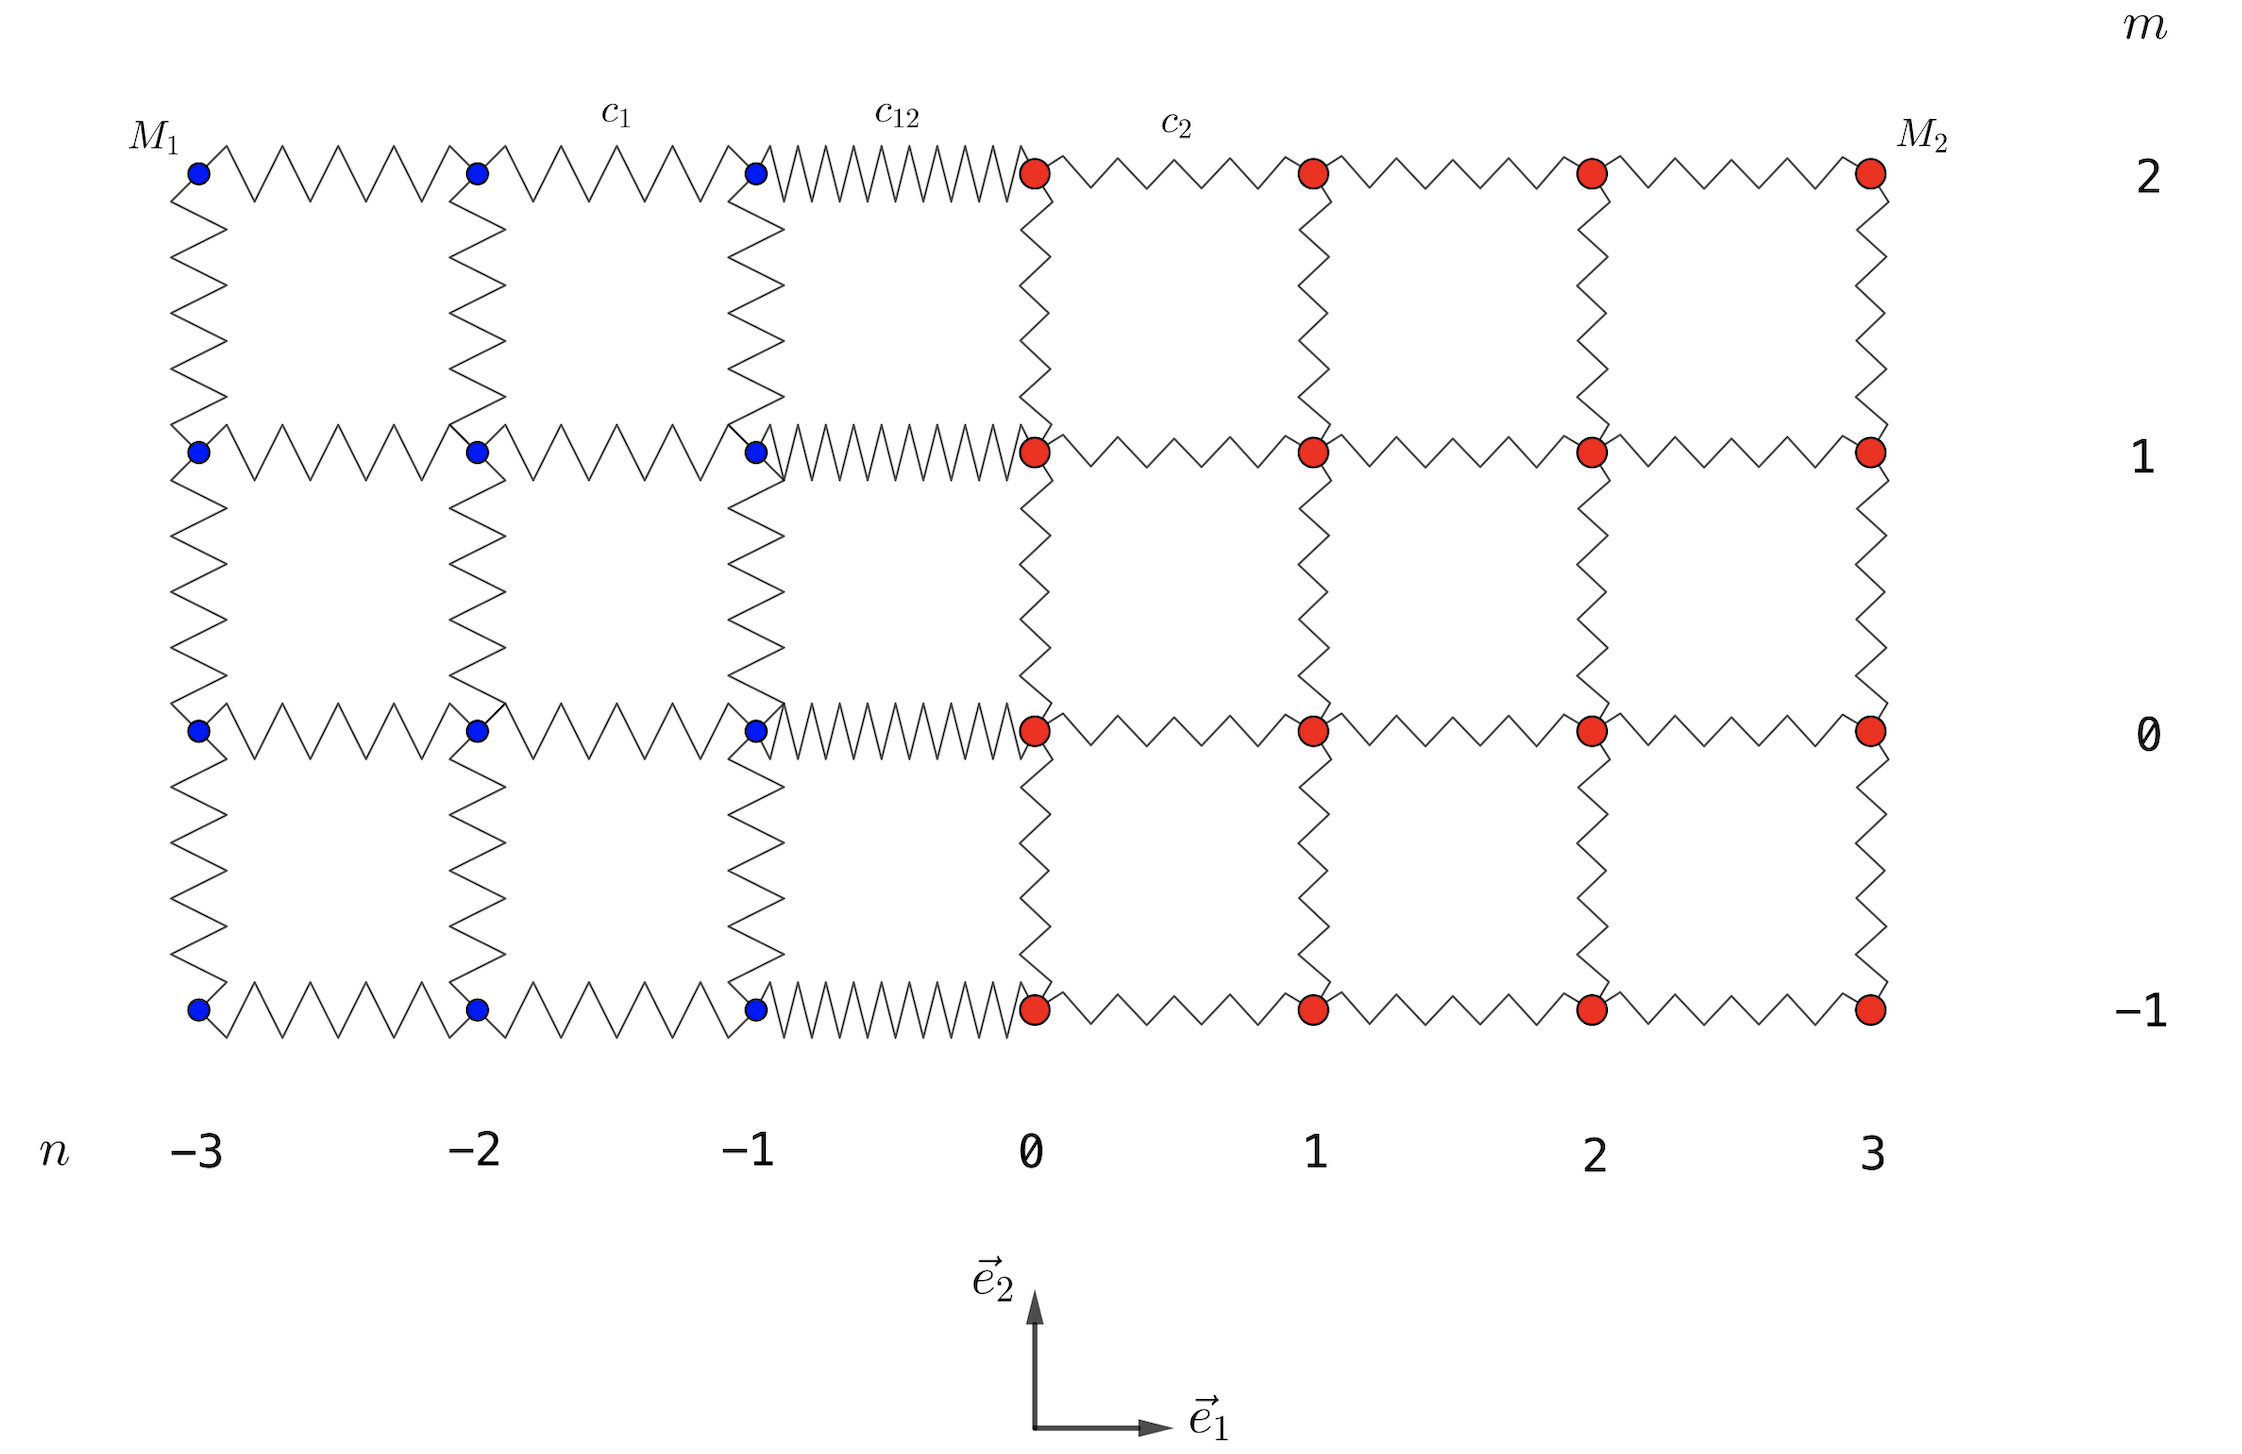
\includegraphics[width=\linewidth]{tex/imgs/lattice-lattice.png}
\caption{Часть рассматриваемой системы двух решёток} 
\label{fig:lattice-lattice}  
\end{figure}

Массы частиц и жёсткости пружин решёток:
\beq
M_{n,m}=
\begin{cases}
M_1, \hspace{0.5cm} n<0,\\
M_2, \hspace{0.5cm} n\geqslant0,
\end{cases}
\hspace{1cm}
C_{n+\frac{1}{2},m}=
\begin{cases}
c_1, \hspace{0.5cm} n<-1,\\
c_{12}, \hspace{0.5cm} n=-1,\\
c_2, \hspace{0.5cm} n\geqslant0,
\end{cases}
\eeq

Уравнение движения для частиц решётки запишется в следующем виде:
\beq
\label{eqn-motion}
M_{n,m}\dot{v}_{n,m}=F_{n+\frac{1}{2},m}-F_{n-\frac{1}{2},m}+F_{n,m+\frac{1}{2}}-F_{n,m-\frac{1}{2}},
\eeq
где
$$
F_{n+\frac{1}{2},m}=C_{n+\frac{1}{2},m}\varepsilon_{n+\frac{1}{2},m}\hspace{2cm}\varepsilon_{n+\frac{1}{2},m}=u_{n+1,m}-u_{n,m}
$$
$$
F_{n,m+\frac{1}{2}}=C_{n,m+\frac{1}{2}}\varepsilon_{n,m+\frac{1}{2}}\hspace{2cm}\varepsilon_{n,m+\frac{1}{2}}=u_{n,m+1}-u_{n,m}
$$

У каждой силы и у каждой жёсткости один индекс целый и один индекс полуцелый.
Положение полуцелого индекса указывает на расположение деформируемой пружины.
Дробный индекс в первой позиции -- деформация пружины, расположенной вдоль оси $Ox$; дробный индекс во второй позиции -- деформация пружины, расположенной вдоль оси $Oy$.

Требуется найти коэффициент прохождения $T$ через границу двух решёток, который определяется как отношение энергии, прошедшей через интерфейс решёток, к суммарной энергии системы.

Требуется методом динамики частиц провести моделирование прохождения волнового пакета через интерфейс при разных углах падения волны на границу двух решёток.
На основе результатов моделирования построить график зависимости коэффициента прохождения (отношения энергии прошедшего волнового пакета к энергии падающего пакета) от угла падения на интерфейс.
И сравнить численные результаты с аналитическим решением.
Сделать выводы.


\subsection{Вывод выражения для коэффициента прохождения волны}

Рассмотрим случай, когда все жёсткости пружин одинаковы, а решётки отличаются только массами частиц.
В этом случае уравнения движения запишутся в следующем виде:
\beq
M_{n,m}\ddot{u}_{n,m}=C\left(u_{n-1,m}+u_{n+1,m}+u_{n,m-1}+u_{n,m+1}-4u_{n,m}\right)
\eeq

Ищем решение уравнений движения в следующем виде (метод трёх волн):
\beq
\label{three-waves}
u_{n,m}=
\begin{cases}
	A_{I}e^{\im\left(\Omega t-ak_1^xn-ak_1^ym\right)}+A_{R}e^{\im\left(\Omega t+ak_1^xn-ak_1^ym\right)},\,\,\,\,\,n<0\\
	A_{T}e^{\im\left(\Omega t-ak_2^xn-ak_2^ym\right)},\,\,\,\,\,n\geqslant 0
\end{cases}
\eeq

Дисперсионное соотношение для решётки:
\beq
\label{disp-rel}
M_i\Omega^2=4C\left(\sin^2{\frac{k_i^xa}{2}}+\sin^2{\frac{k_i^ya}{2}}\right)
\eeq

\begin{figure}[H] 
\center
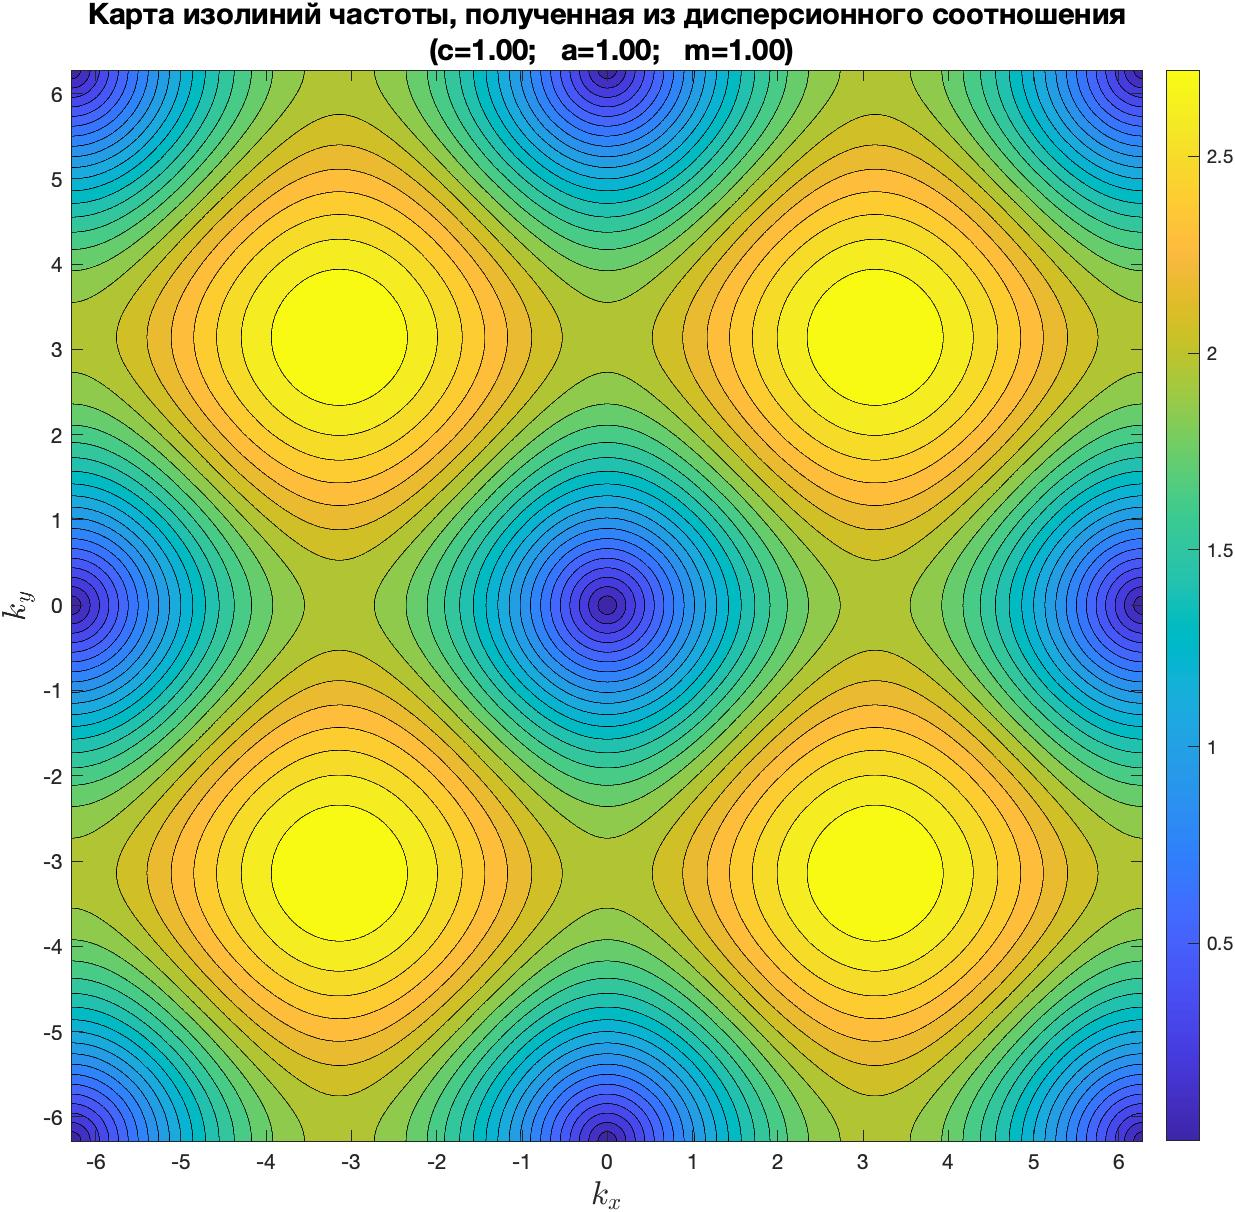
\includegraphics[width=.4\linewidth]{tex/imgs/lattice-dispersion-relation.jpg}
\caption{Карта изолиний частоты полученная из дисперсионного соотношения} 
\label{fig:lattice-dispersion-relation}  
\end{figure}

Уравнения движения для частиц интерфейса:
\beq
\label{interface-move}
\begin{cases}
	M_1\ddot{u}_{-1,m}=c\left(u_{0,m}+u_{-1,m+1}+u_{-2,m}+u_{-1,m-1}-4u_{-1,m}\right)\\
	M_2\ddot{u}_{0,m}=c\left(u_{1,m}+u_{0,m+1}+u_{-1,m}+u_{0,m-1}-4u_{0,m}\right)
\end{cases}
\eeq

Подставляем \eqref{three-waves} в \eqref{interface-move}:
\beq
\begin{cases}
\begin{aligned}
-M_1\Omega^2\left(A_Ie^{\im a\left(k_1^x-k_1^ym\right)}+A_Re^{\im a\left(-k_1^x-k_1^ym\right)}\right)=C&\left[A_Te^{-\im ak_2^ym}+A_Ie^{\im a\left(k_1^x-k_1^y(m+1)\right)}\right.+\\
&+\left.A_Re^{\im a\left(-k_1^x-k_1^y(m+1)\right)}+A_Ie^{\im a\left(2k_1^x-k_1^ym\right)}\right.+\\
&+\left.A_Re^{\im a\left(-2k_1^x-k_1^ym\right)}+A_Ie^{\im a\left(k_1^x-k_1^y(m-1)\right)}\right.+\\
&+\left.A_Re^{\im a\left(-k_1^x-k_1^y(m-1)\right)}\right.-\\
&-\left.4\left(A_Ie^{\im a\left(k_1^x-k_1^ym\right)}+A_Re^{\im a\left(-k_1^x-k_1^ym\right)}\right)\right]
\end{aligned}\\\\
\begin{aligned}
-M_2\Omega^2\left(A_Te^{-\im ak_2^ym}\right)=C&\left[A_Te^{\im a\left(-k_2^x-k_2^ym\right)}+A_Te^{-\im ak_2^y(m+1)}+A_Ie^{\im a\left(k_1^x-k_1^ym\right)}\right.+\\
&+\left.A_Re^{\im a\left(-k_1^x-k_1^ym\right)}+A_Te^{-\im ak_2^y(m-1)}-4A_Te^{-\im ak_2^ym}\right]
\end{aligned}
\end{cases}
\eeq

Преобразуем, используя дисперсионное соотношение \eqref{disp-rel}:
\beq
\begin{cases}
\begin{aligned}
\left(e^{\im k_1^xa}+e^{-\im k_1^xa}+e^{\im k_1^y a}+e^{-\im k_1^ya}-4\right)&\left(A_Ie^{\im a\left(k_1^x-k_1^ym\right)}+A_Re^{\im a\left(-k_1^x-k_1^ym\right)}\right)=\\
&=A_Te^{-\im ak_2^ym}+A_Ie^{\im a\left(k_1^x-k_1^y(m+1)\right)}+\\
&+A_Re^{\im a\left(-k_1^x-k_1^y(m+1)\right)}+A_Ie^{\im a\left(2k_1^x-k_1^ym\right)}+\\
&+A_Re^{\im a\left(-2k_1^x-k_1^ym\right)}+A_Ie^{\im a\left(k_1^x-k_1^y(m-1)\right)}+\\
&+A_Re^{\im a\left(-k_1^x-k_1^y(m-1)\right)}-\\
&-4\left(A_Ie^{\im a\left(k_1^x-k_1^ym\right)}+A_Re^{\im a\left(-k_1^x-k_1^ym\right)}\right)
\end{aligned}\\\\
\begin{aligned}
\left(e^{\im k_2^x a}+e^{-\im k_2^xa}+e^{\im k_2^ya}+e^{-\im k_2^y a}-4\right)&\left(A_Te^{-\im ak_2^ym}\right)=\\
&=A_Te^{\im a\left(-k_2^x-k_2^ym\right)}+A_Te^{-\im ak_2^y(m+1)}+A_Ie^{\im a\left(k_1^x-k_1^ym\right)}+\\
&+A_Re^{\im a\left(-k_1^x-k_1^ym\right)}+A_Te^{-\im ak_2^y(m-1)}-4A_Te^{-\im ak_2^ym}
\end{aligned}
\end{cases}
\eeq

Далее преобразуем:
\beq
\begin{cases}
\left(A_I+A_R\right)e^{-\im ak_1^ym}=A_Te^{-\im ak_2^ym}\\
A_Ie^{\im a\left(k_1^x-k_1^ym\right)}+A_Re^{-\im a\left(k_1^x+k_1^ym\right)}=A_Te^{\im a\left(k_2^x-k_2^ym\right)}
\end{cases}
\eeq

Получаем:
\beq
\frac{A_T}{A_I}=\frac{e^{\im a\left(k_1^x-k_1^ym\right)}-e^{-\im a\left(k_1^x+k_1^ym\right)}}{e^{\im a\left(k_2^x-k_2^ym\right)}-e^{-\im a\left(k_1^x+k_2^ym\right)}}
\eeq

Или:
\beq
\frac{A_T}{A_I}=\frac{e^{\im k_1^xa}-e^{-\im k_1^xa}}{e^{\im k_2^xa}-e^{-\im k_1^xa}}\cdot\frac{e^{\im k_2^y am}}{e^{\im k_1^y am}}
\eeq

Тогда:
\beq
\left|\frac{A_T}{A_I}\right|=\left|\frac{e^{\im k_1^xa}-e^{-\im k_1^xa}}{e^{\im k_2^xa}-e^{-\im k_1^xa}}\right|\cdot\left|\frac{e^{\im k_2^y am}}{e^{\im k_1^y am}}\right|=\left|\frac{e^{\im k_1^xa}-e^{-\im k_1^xa}}{e^{\im k_2^xa}-e^{-\im k_1^xa}}\right|
\eeq

Таким образом,
\beq
T=\frac{M_2g_2^x}{M_1g_1^x}\left|\frac{e^{\im k_1^xa}-e^{-\im k_1^xa}}{e^{\im k_2^xa}-e^{-\im k_1^xa}}\right|^2,
\eeq
где
$$
g_i=\frac{d\Omega}{dk_i};\hspace{2cm}g_i^x=g_i\cos{\gamma};\hspace{2cm}g_i^y=g_i\sin{\gamma}.
$$

Далее вводится предположение, что при прохождении через интерфейс $Oy$-компонента волнового вектора не меняется $\left(k_1^y=k_2^y\right)$.
И с помощью следующего кода определяется коэффициент прохождения волны:

\begin{pythoncode}
import numpy as np
from numpy import sin, cos
from scipy.optimize import fsolve
import sympy as sp
from sympy import Symbol, Abs, I, exp, diff
from sympy.plotting import plot


def transmission_analytical(m_1, m_2, c, omega, a, gamma):

    # find wave vector components (in lattice 1) that corresponds to given frequency omega and angle gamma
    k1 = fsolve(lambda k: m_1*omega**2-4*c*(sin(cos(gamma)*k*a/2)**2+sin(sin(gamma)*k*a/2)**2), 1)[0]
    k1_x = k1*cos(gamma)
    k1_y = k1*sin(gamma)

    # find wave vector components (in lattice 2) and refraction angle using Snell's law
    k2_y = k1_y
    k2_x = fsolve(lambda k: m_2*omega**2-4*c*(sin(k*a/2)**2+sin(k2_y*a/2)**2), 0.5)[0]
    k2 = np.sqrt(k2_x**2+k2_y**2)
    zeta = np.arctan(k2_y/k2_x)

    # find group velocities
    k = Symbol('k')
    g1 = diff(2*np.sqrt(c/m_1)*sp.sqrt(sp.sin(k*np.cos(gamma)*a/2)**2+\
                                       sp.sin(k*np.sin(gamma)*a/2)**2),k).evalf(subs={k:k1})
    g1_x = g1*np.cos(gamma)
    g1_y = g1*np.sin(gamma)
    g2 = diff(2*np.sqrt(c/m_2)*sp.sqrt(sp.sin(k*np.cos(zeta)*a/2)**2+\
                                       sp.sin(k*np.sin(zeta)*a/2)**2),k).evalf(subs={k:k2})
    g2_x = g2*np.cos(zeta)
    g2_y = g2*np.sin(zeta)

    A_frac = (exp(I*k1_x*a)-exp(-I*k1_x*a))/(exp(I*k2_x*a)-exp(-I*k1_x*a))
    A_frac = A_frac.evalf()
    trans_coeff = m_2*g2_x/(m_1*g1_x)*(Abs(A_frac))**2
    
    return trans_coeff
\end{pythoncode}

Сравнение полученных результатов с численным моделированием будет представлено далее.



\subsection{Численное решение}

Моделирование проводится только для случая одинаковых жёсткостей пружин: $c_1=c_2=c_{12}=C$ (жёсткости пружин левой решётки, жёсткости пружин правой решётки и жёсткости пружин интерфейса совпадают).

Уравнение движения частицы $\left(n,m\right)$ запишется в следующем виде:
\beq
M_{n,m}\ddot{u}_{n,m}=C\left(u_{n+1,m}+u_{n,m+1}+u_{n-1,m}+u_{n,m-1}-4u_{n,m}\right)
\eeq

Начальные условия (для перемещений и скоростей частиц) заданы в виде волнового пакета:
\beq
\begin{aligned}
u_{n,m}^0=u_0&\exp{\left(-\frac{\beta_x}{2}\left[(n-n_0)\cos{\gamma}+(m-m_0)\sin{\gamma}\right]^2\right)}\\
&\exp{\left(-\frac{\beta_y^2}{2}\left[(-n+n_0)\sin{\gamma}+(m-m_0)\cos{\gamma}\right]^2\right)}\\
&\sin{\left(k_1a(n\cos{\gamma}+m\sin{\gamma})\right)}
\end{aligned}
\eeq

\beq
\begin{aligned}
v_{n,m}^0=-u_0&\exp{\left(-\frac{\beta_x}{2}\left[(n-n_0)\cos{\gamma}+(m-m_0)\sin{\gamma}\right]^2\right)}\\
&\exp{\left(-\frac{\beta_y^2}{2}\left[(-n+n_0)\sin{\gamma}+(m-m_0)\cos{\gamma}\right]^2\right)}\\
&\bigg(\Omega\cos{\!\left(k_1a(n\cos{\gamma}+m\sin{\gamma})\right)}-\\
&-\left.\frac{\beta_x^2g_1}{a}\left[(n-n_0)\cos{\gamma}+m\sin{\gamma}\right]\,\sin{\!\left(k_1a(n\cos{\gamma}+m\sin{\gamma})\right)}\right)
\end{aligned}
\eeq

На границах заданы периодические граничные условия.

Интегрирование уравнений движения проводится методом leap-frog:
\beq
\begin{aligned}
a_{n,m}^{t}&=\frac{C}{M}\left(u_{n+1,m}^t+u_{n,m+1}^t+u_{n-1,m}^t+u_{n,m-1}^t-4u_{n,m}^t\right)\\
u_{n,m}^{t+\Delta t}&=u_{n,m}^{t}+v_{n,m}^{t}\Delta t+\frac{a_{n,m}^{t}(\Delta t)^2}{2}\\
a_{n,m}^{t+\Delta t}&=\frac{C}{M}\left(u_{n+1,m}^{t+\Delta t}+u_{n,m+1}^{t+\Delta t}+u_{n-1,m}^{t+\Delta t}+u_{n,m-1}^{t+\Delta t}-4u_{n,m}^{t+\Delta t}\right)\\
v_{n,m}^{t+\Delta t}&=v_{n,m}^t+\frac{1}{2}\left(a_{n,m}^{t}+a_{n,m}^{t+\Delta t}\right)\Delta t
\end{aligned}
\eeq

Энергия вычисляется по формуле:
\beq
\begin{aligned}
e_{n,m}=\frac{M v_{n,m}^2}{2}+\frac{C}{4}&\left(\left(u_{n+1,m}-u_{n,m}\right)^2+\left(u_{n-1,m}-u_{n,m}\right)^2+\right.\\
&\left.+\left(u_{n,m+1}-u_{n,m}\right)^2+\left(u_{n,m-1}-u_{n,m}\right)^2\right)
\end{aligned}
\eeq

Далее представлены результаты моделирования прохождения волны через интерфейс двух решёток.

\begin{figure}[H] 
\center
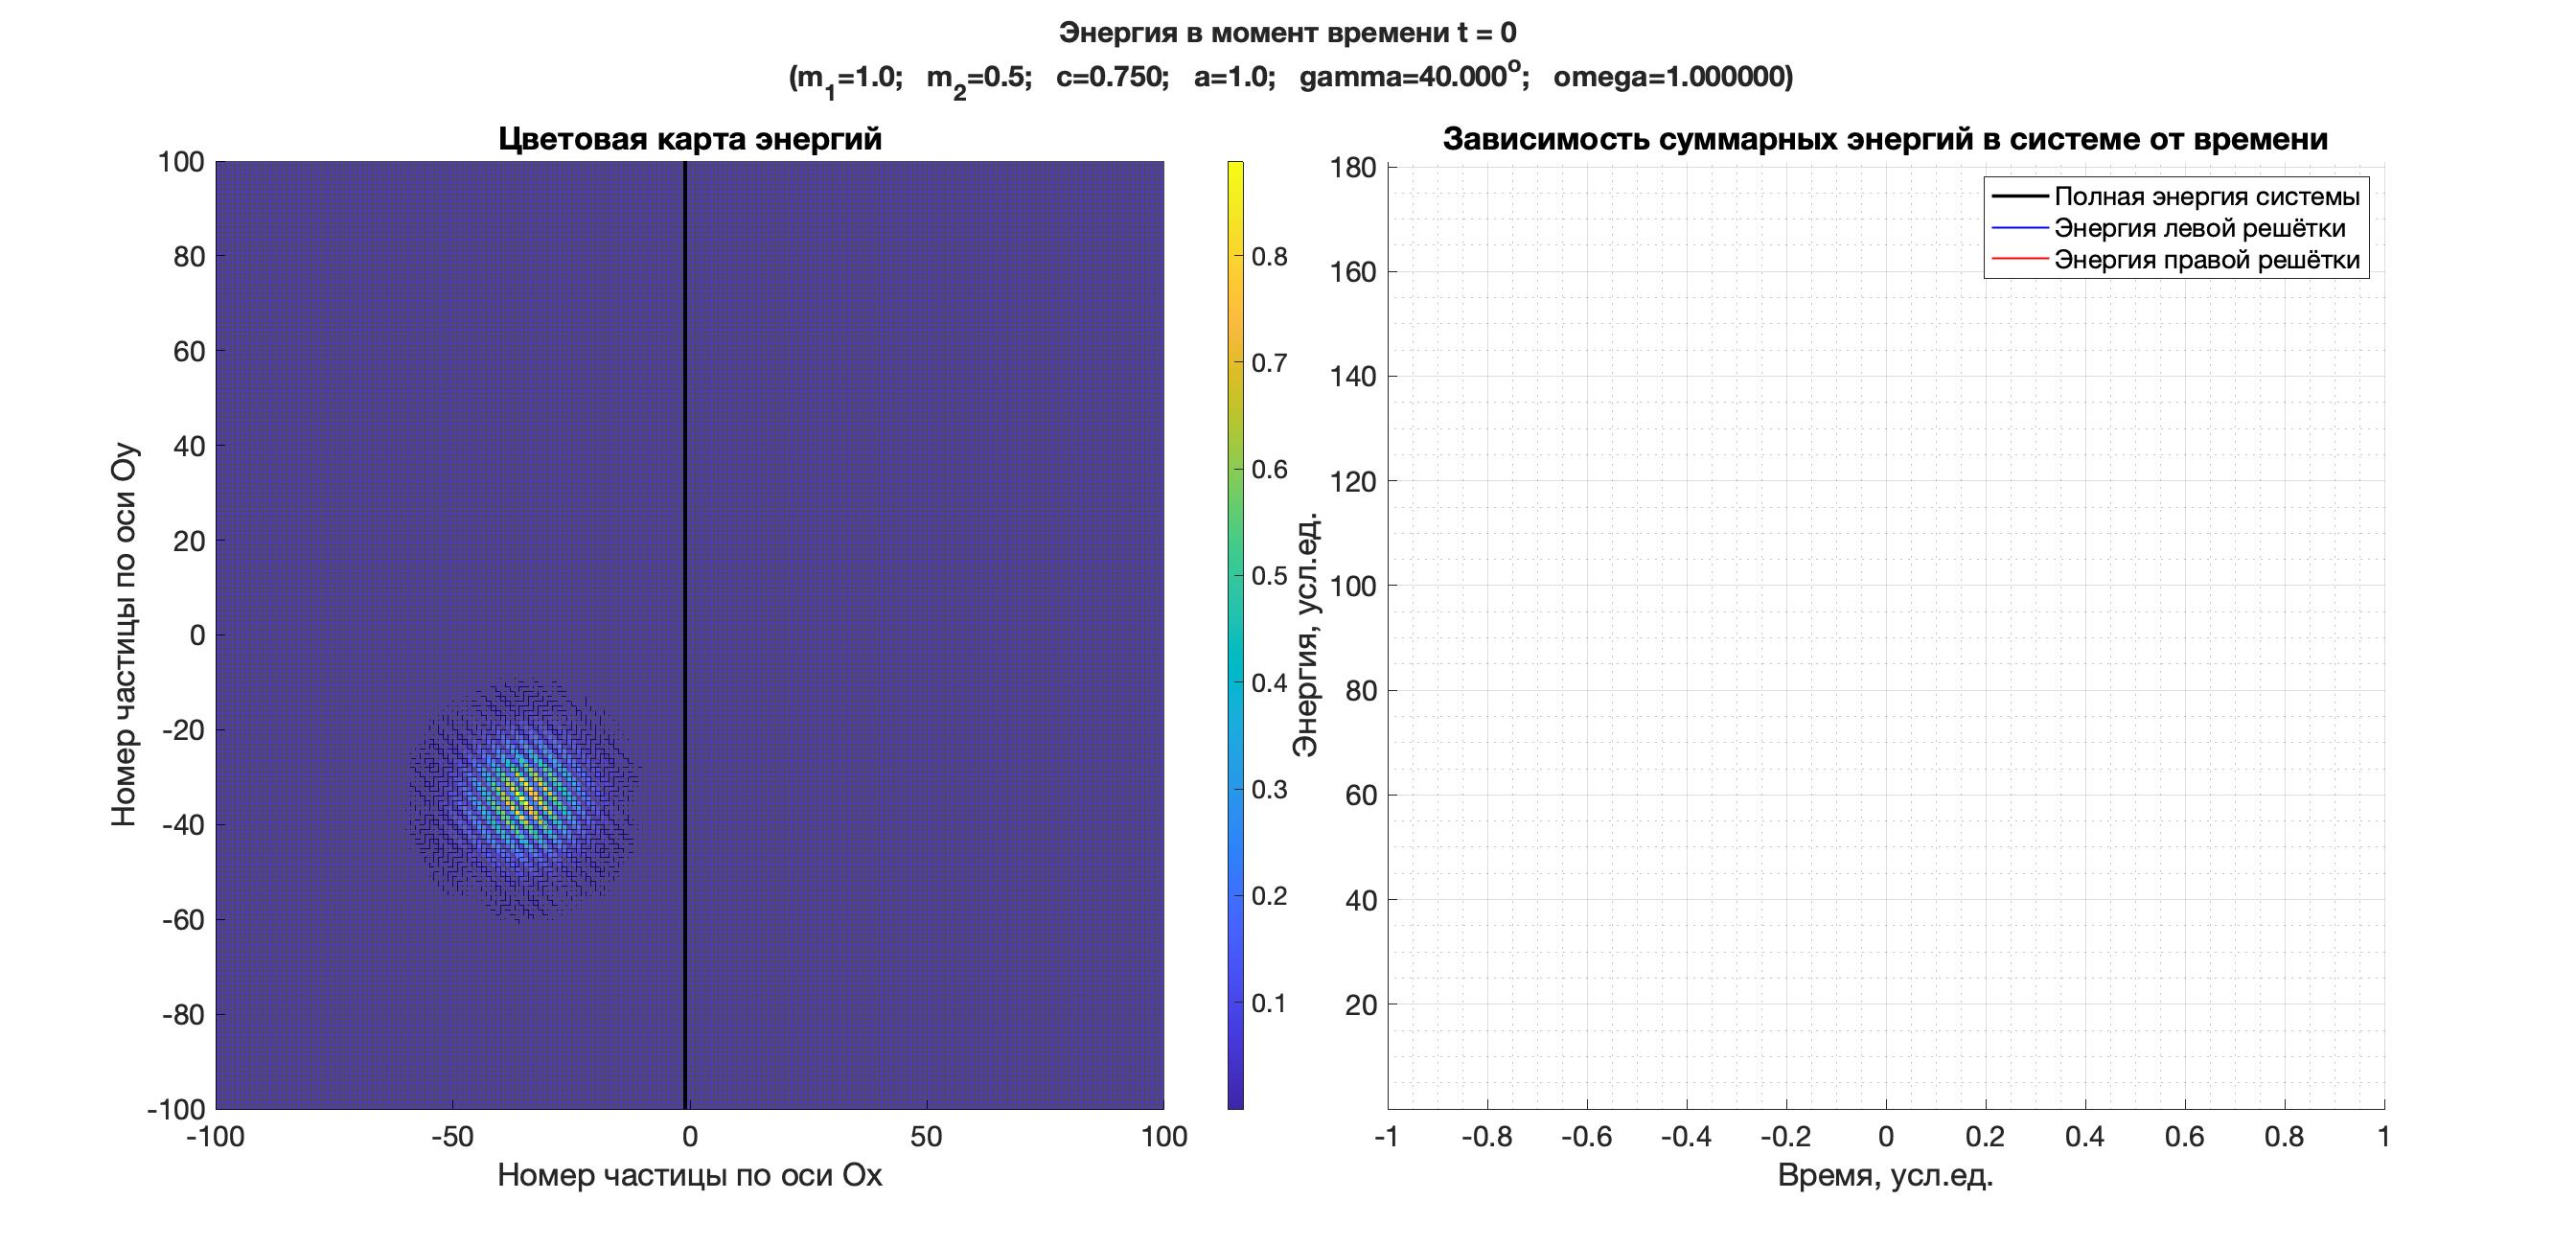
\includegraphics[width=\linewidth]{tex/imgs/modelling-0.jpg}
\caption{Распределение энергии в начальный момент времени} 
\label{fig:modelling-0}  
\end{figure}

\begin{figure}[H] 
\center
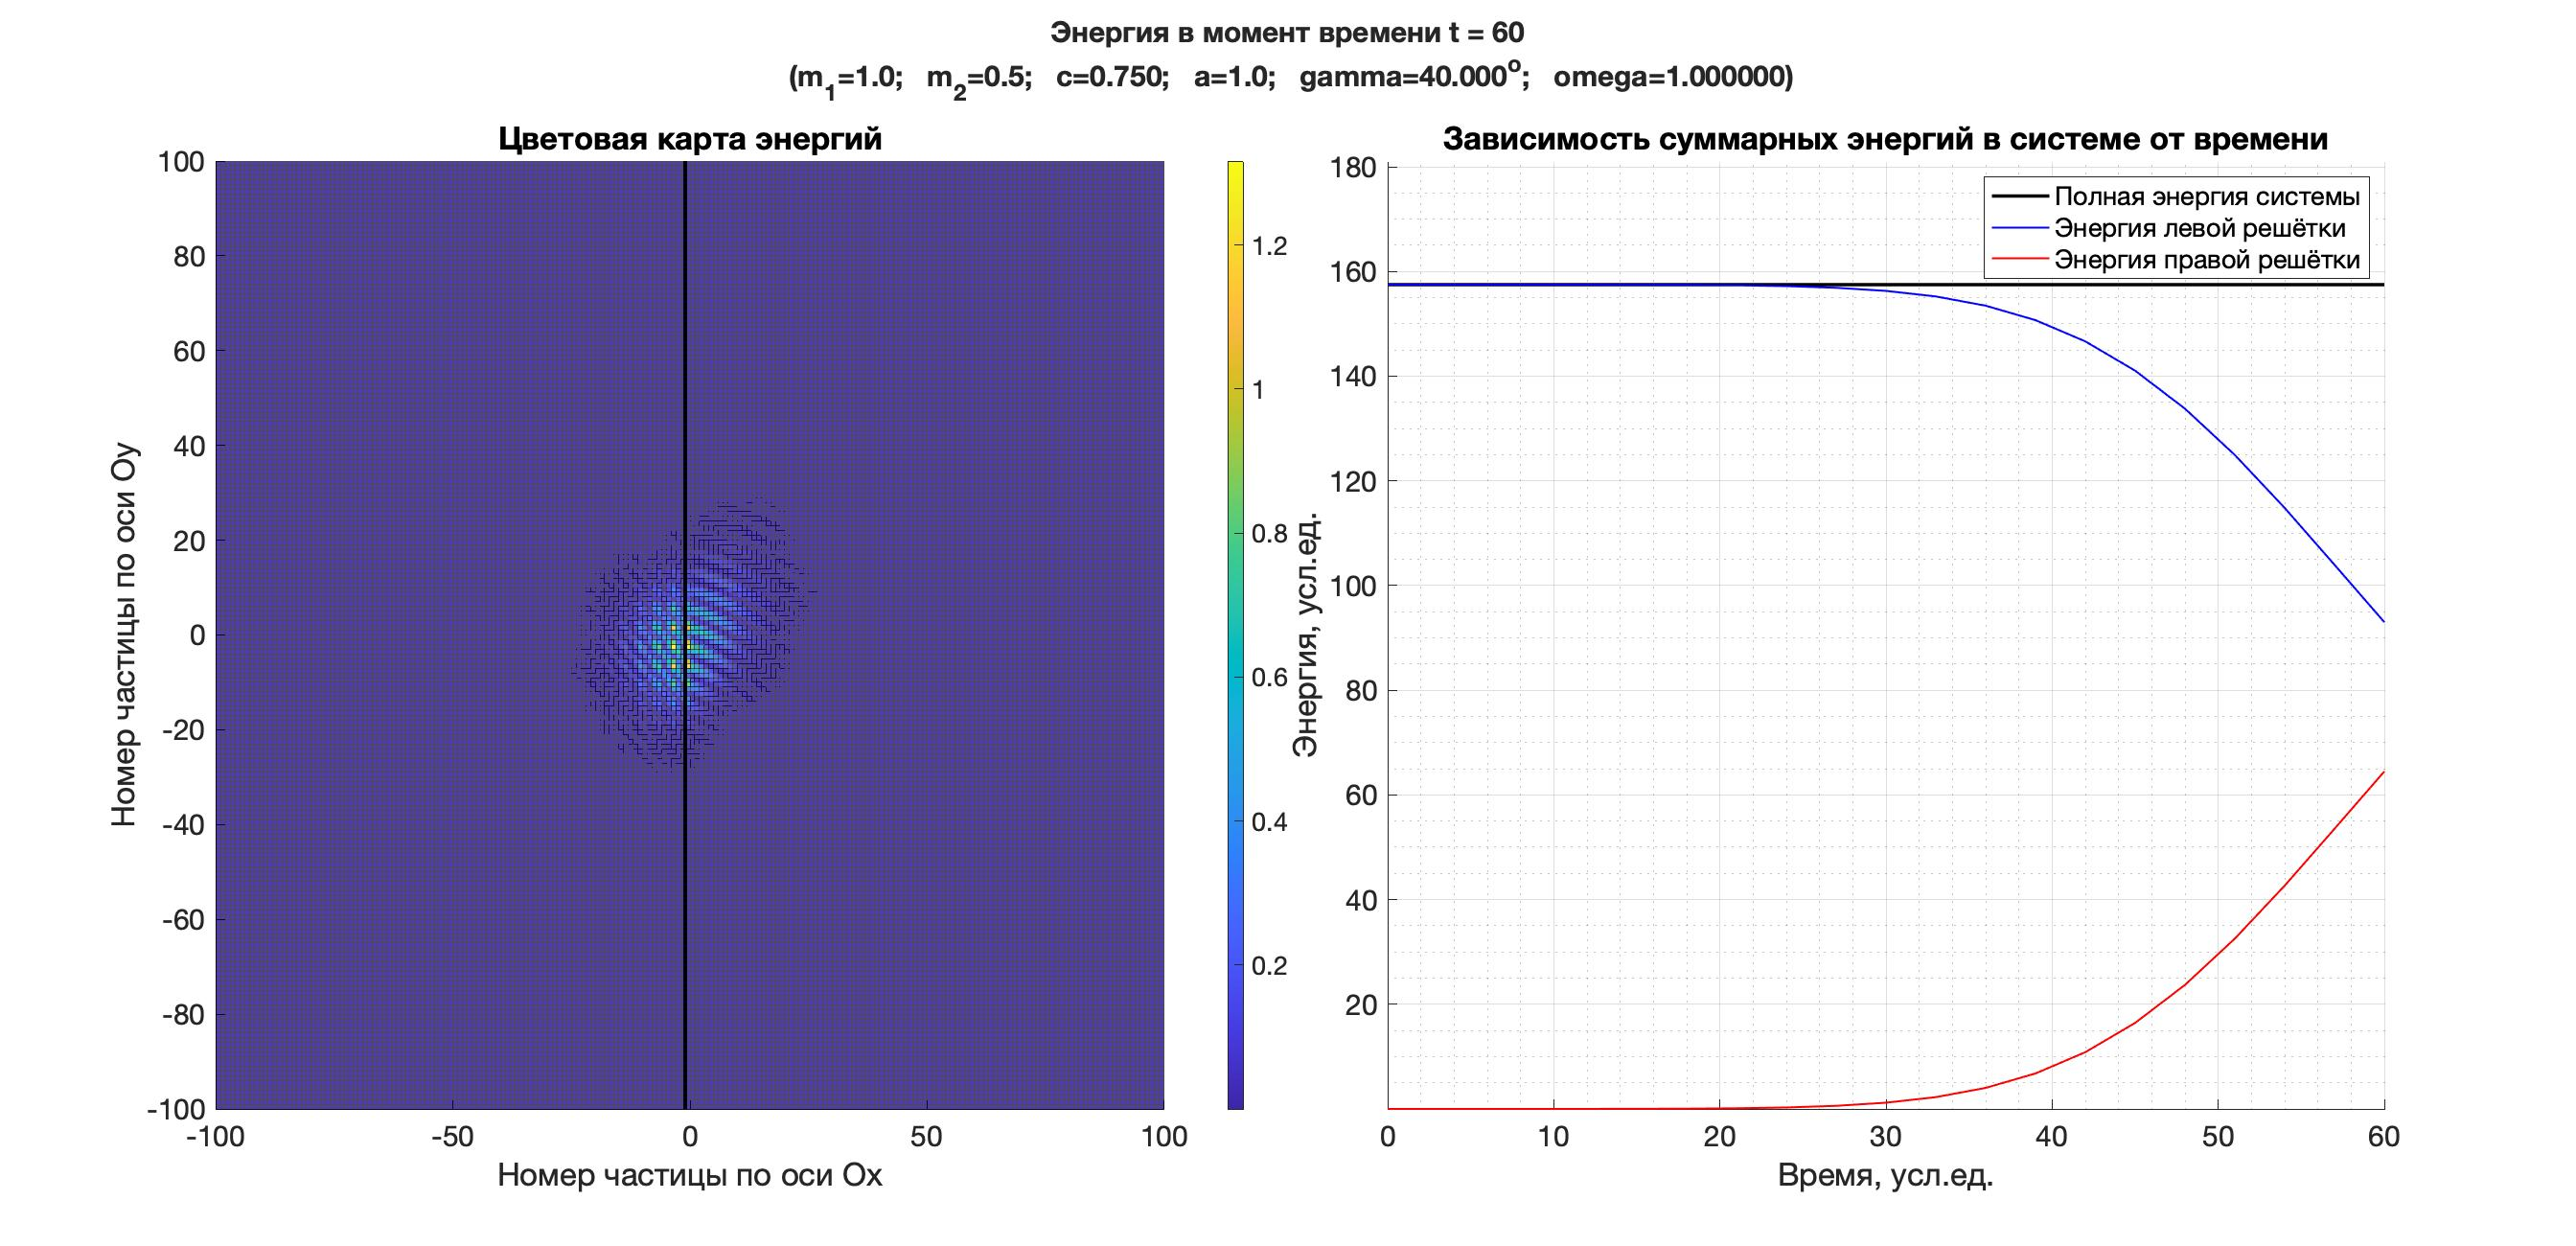
\includegraphics[width=\linewidth]{tex/imgs/modelling-1.jpg}
\caption{Распределение энергии в момент времени $t=60$ усл.ед.}
\label{fig:modelling-1}  
\end{figure}

Из рис. \ref{fig:modelling-1} видим, что суммарная энергия в левой решётке уменьшается, а в правой -- увеличивается.

\begin{figure}[H] 
\center
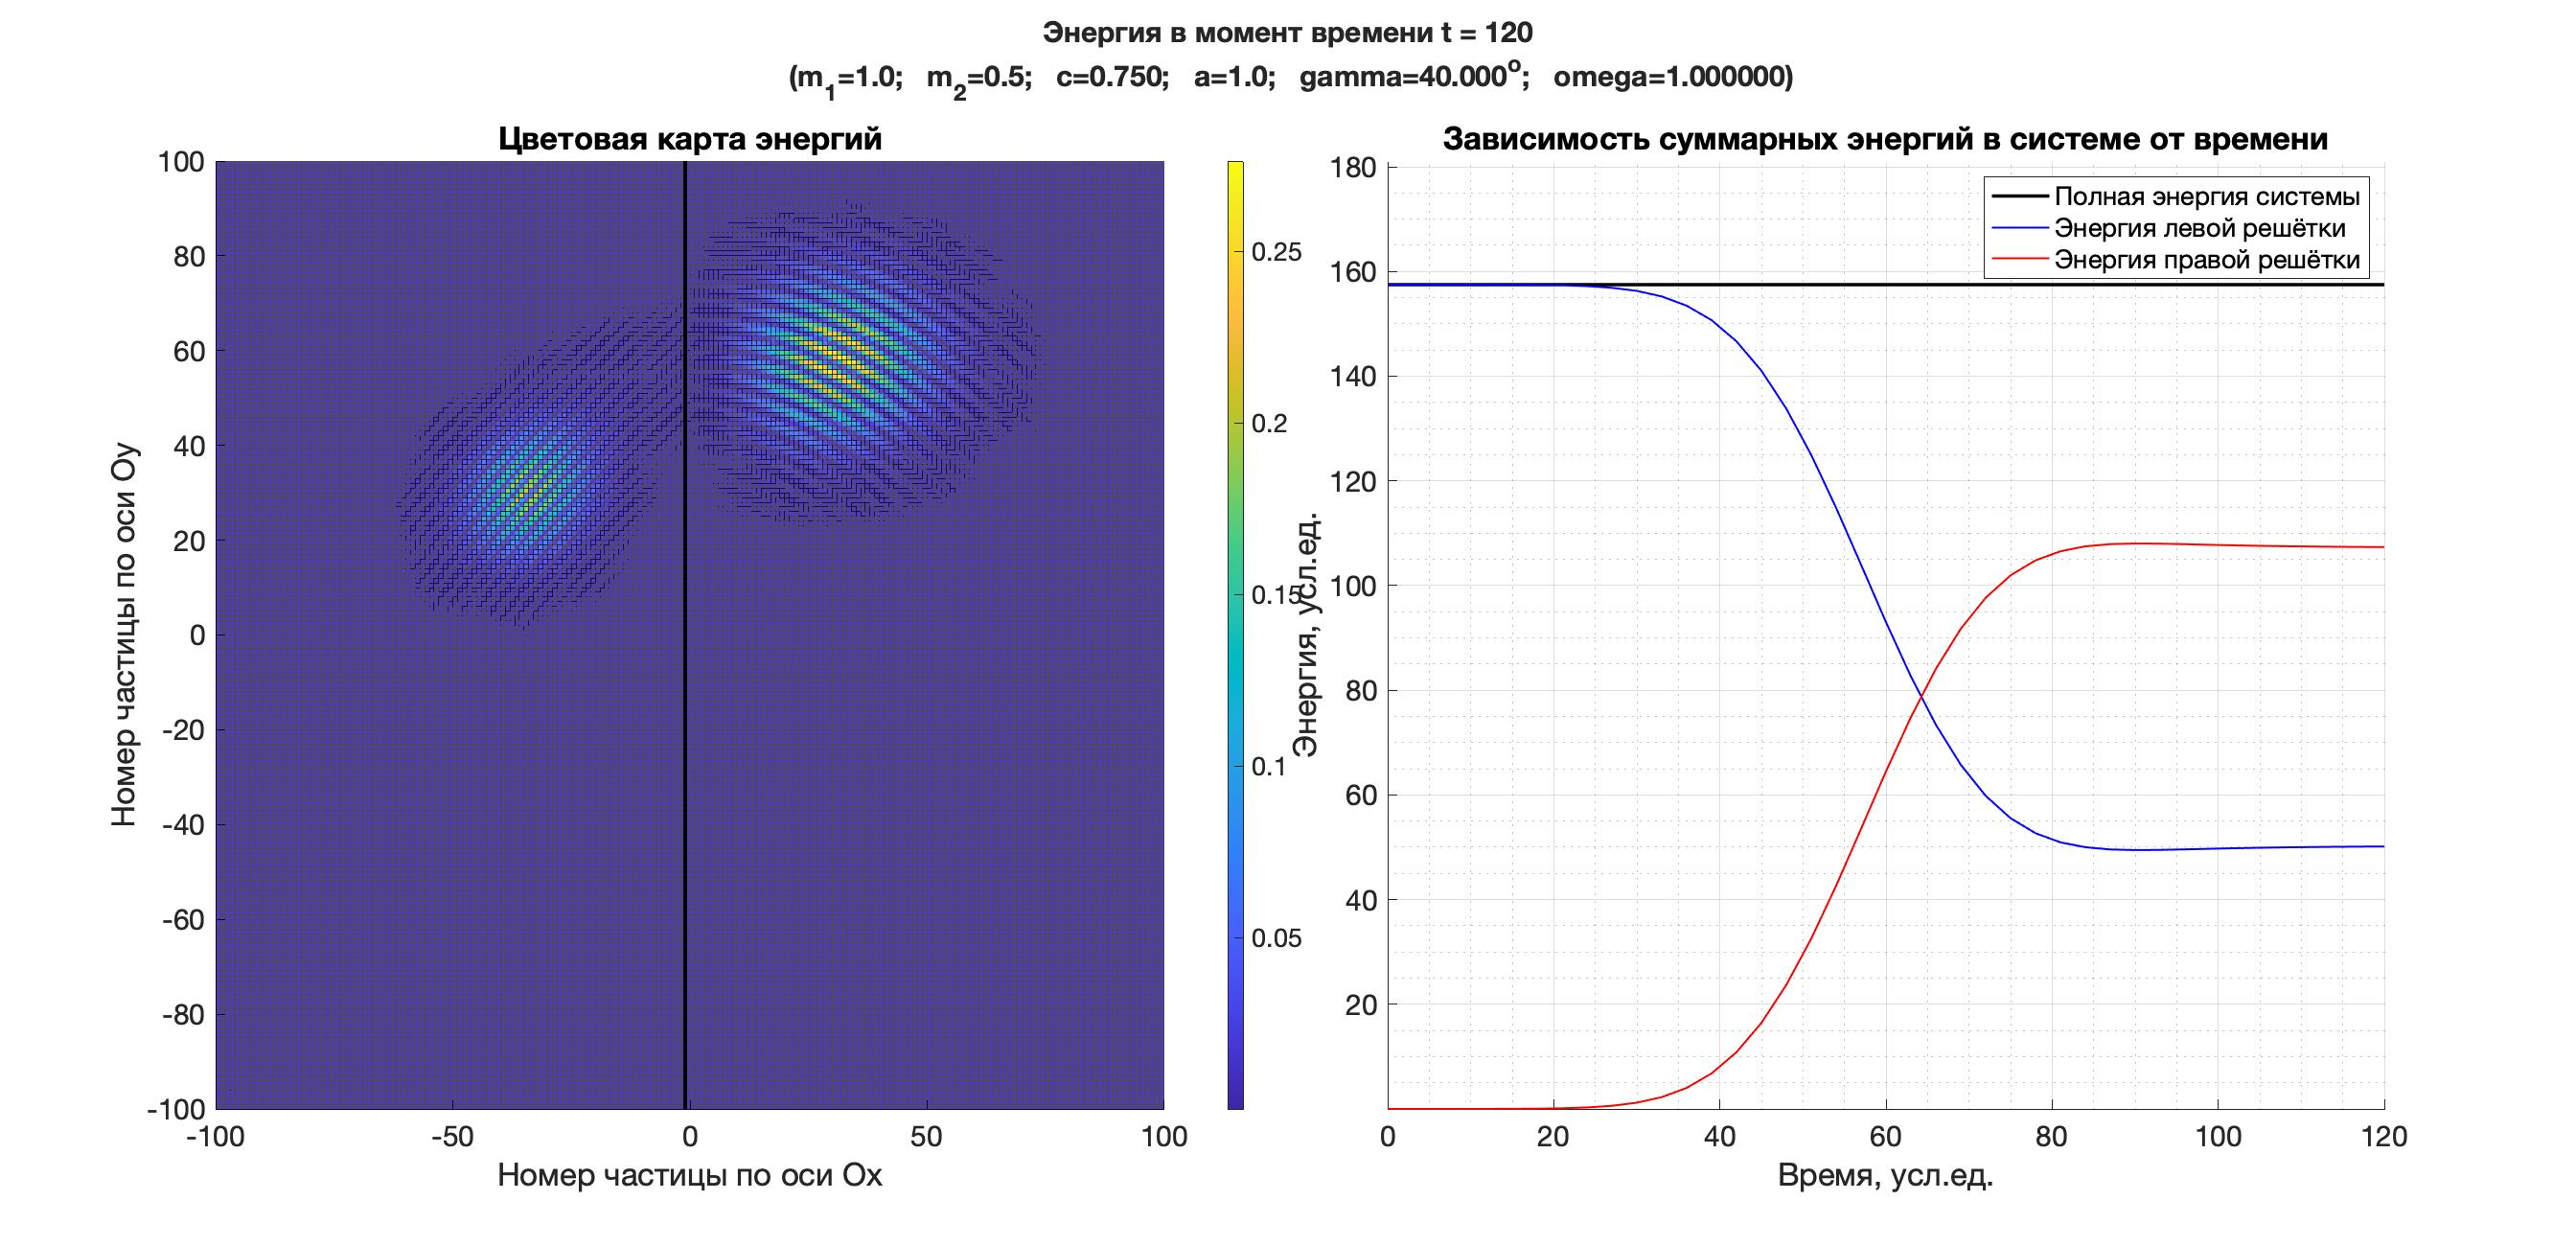
\includegraphics[width=\linewidth]{tex/imgs/modelling-2.jpg}
\caption{Распределение энергии в момент времени $t=120$ усл.ед.}
\label{fig:modelling-2}  
\end{figure}

Из рис. \ref{fig:modelling-2} видим, что волна прошла во вторую решётку и частично отразилась от интерфейса.

\begin{figure}[H] 
\center
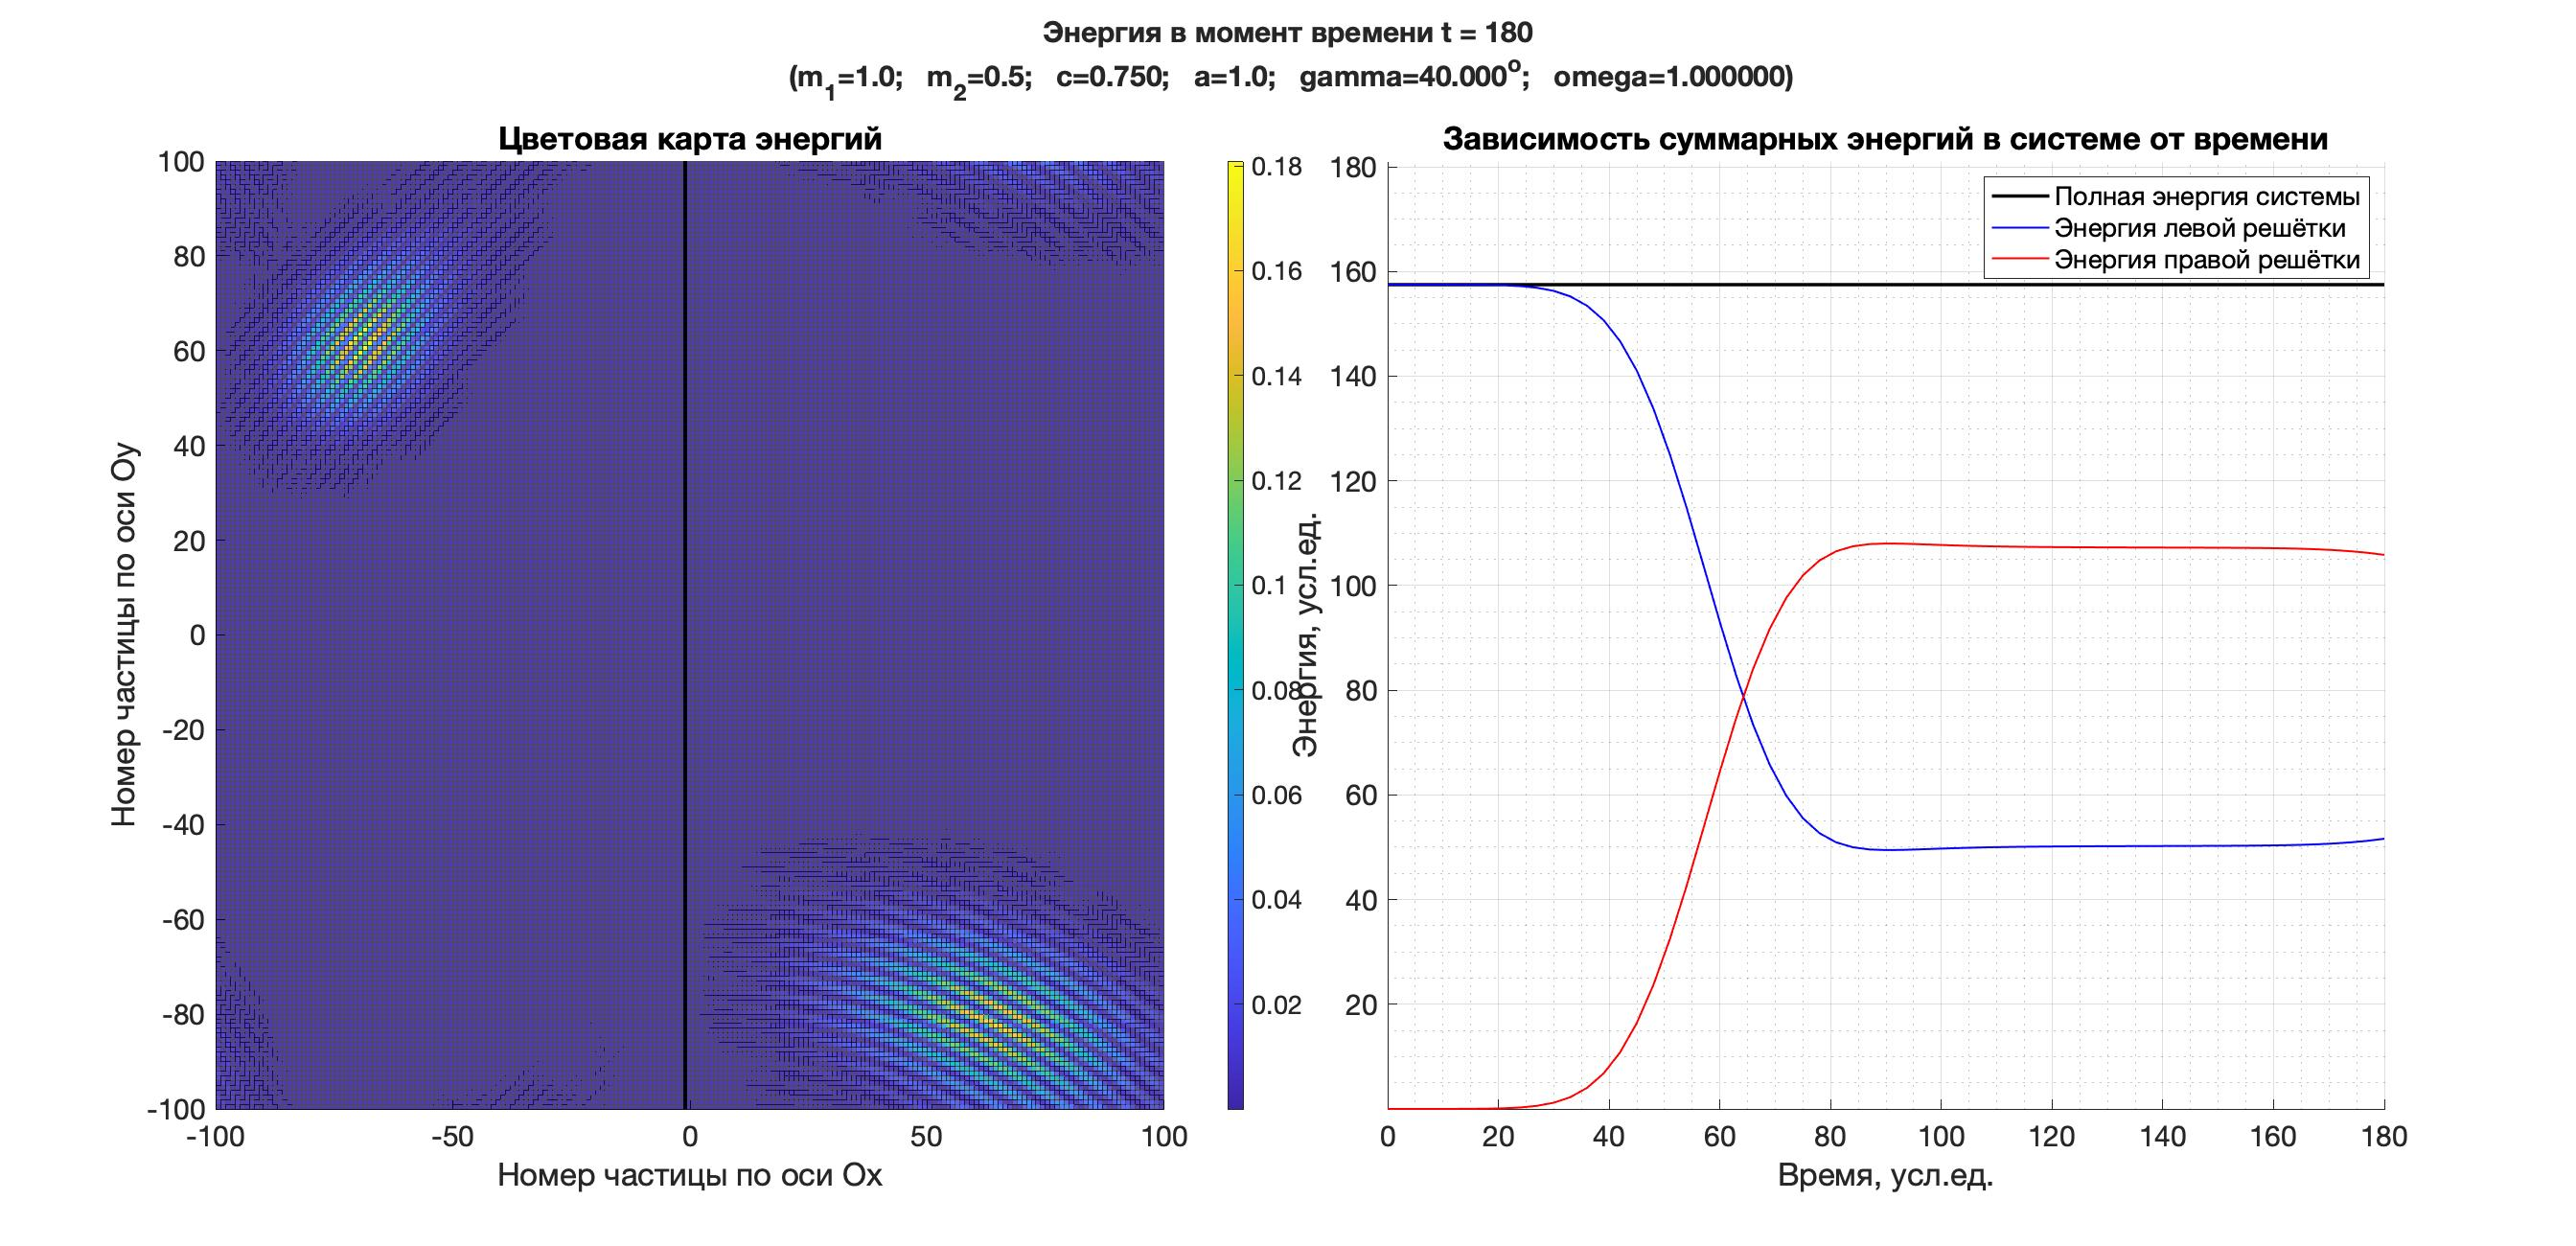
\includegraphics[width=\linewidth]{tex/imgs/modelling-3.jpg}
\caption{Распределение энергии в момент времени $t=180$ усл.ед.}
\label{fig:modelling-3}  
\end{figure}

Далее запустим аналогичный эксперимент при разных углах падения волны на интерфейс двух решёток и построим график зависимости коэффициента прохождения в зависимости от угла падения.
На этом же графике построим зависимость, полученную аналитически.

\begin{figure}[H] 
\center
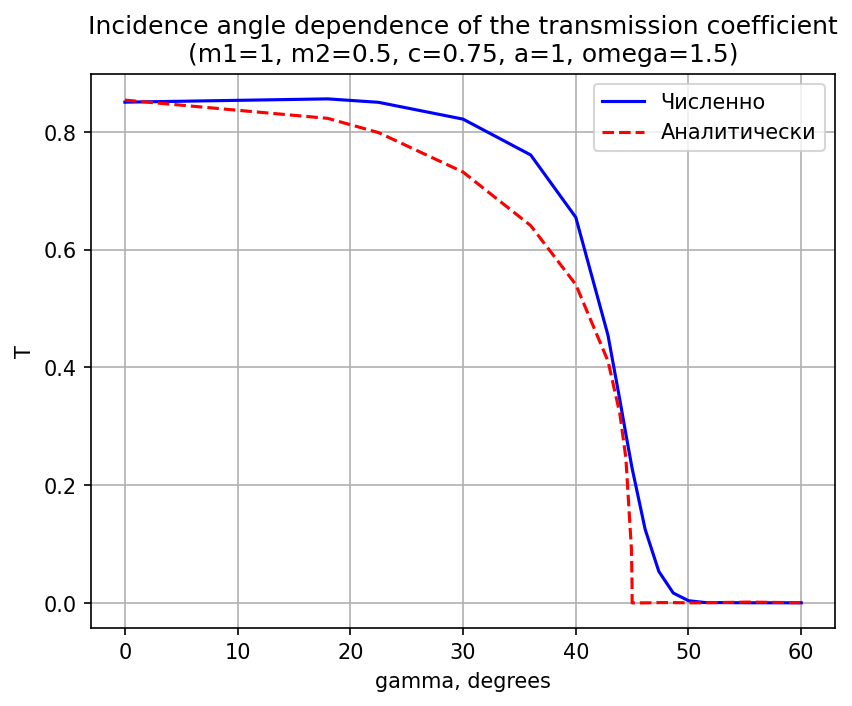
\includegraphics[width=.6\linewidth]{tex/imgs/transmission-coefficient.png}
\caption{Зависимость коэффициента прохождения от угла падения волны на интерфейс двух решёток} 
\label{fig:transmission-coefficient}  
\end{figure}

Из рис. \ref{fig:transmission-coefficient} видим, что численное и аналитическое решения дают разные результаты.
Скорее всего это связано с тем, что при выводе аналитического решения было использовано предположение о сохранении $Oy$-компоненты волнового вектора при прохождении через интерфейс.
В дальнейшем требуется найти, каким образом изменяется $Oy$-компонента волнового вектора при прохождении через интерфейс двух решёток.

\subsection{Поиск производной суммарного потока энергии в решётках}

В этом разделе масса частиц левой решётки $M_1$, жёсткость пружин левой решётки $c_1$; масса частиц правой решётки $M_2$, жёсткость пружин правой решётки $c_2$; жёсткость пружин интерфейса $c_{12}$.

Уравнение движения для частицы $\left(n,m\right)$:
\beq
\label{eqn-motion}
M_{n,m}\dot{v}_{n,m}=F_{n+\frac{1}{2},m}-F_{n-\frac{1}{2},m}+F_{n,m+\frac{1}{2}}-F_{n,m-\frac{1}{2}},
\eeq
где
$$
F_{n+\frac{1}{2},m}=C_{n+\frac{1}{2},m}\varepsilon_{n+\frac{1}{2},m}\hspace{2cm}\varepsilon_{n+\frac{1}{2},m}=u_{n+1,m}-u_{n,m}
$$
$$
F_{n,m+\frac{1}{2}}=C_{n,m+\frac{1}{2}}\varepsilon_{n,m+\frac{1}{2}}\hspace{2cm}\varepsilon_{n,m+\frac{1}{2}}=u_{n,m+1}-u_{n,m}
$$

Выражение для потока энергии:
\beq
\uline{h}_{n+\frac{1}{2},m+\frac{1}{2}}=-\frac{a\uline{e_1}}{2}F_{n+\frac{1}{2},m}\left(v_{n+1,m}+v_{n,m}\right)-\frac{a\uline{e_2}}{2}F_{n,m+\frac{1}{2}}\left(v_{n,m+1}+v_{n,m}\right)
\eeq

Производная потока энергии:
\beq
\label{flux-der}
\begin{aligned}
\uline{\dot{h}}_{n+\frac{1}{2},m+\frac{1}{2}}=
&-\frac{a\uline{e_1}}{2}\dot{F}_{n+\frac{1}{2},m}\left(v_{n+1,m}+v_{n,m}\right)-\\[1ex]
&-\frac{a\uline{e_1}}{2}F_{n+\frac{1}{2},m}\left(\dot{v}_{n+1,m}+\dot{v}_{n,m}\right)-\\[1ex]
&-\frac{a\uline{e_2}}{2}\dot{F}_{n,m+\frac{1}{2}}\left(v_{n,m+1}+v_{n,m}\right)-\\[1ex]
&-\frac{a\uline{e_2}}{2}F_{n,m+\frac{1}{2}}\left(\dot{v}_{n,m+1}+\dot{v}_{n,m}\right).
\end{aligned}
\eeq

Из уравнения движения \eqref{eqn-motion}:
\beq
\label{vels}
\begin{aligned}
\dot{v}_{n,m}&=\frac{F_{n+\frac{1}{2},m}}{M_{n,m}}-\frac{F_{n-\frac{1}{2},m}}{M_{n,m}}+\frac{F_{n,m+\frac{1}{2}}}{M_{n,m}}-\frac{F_{n,m-\frac{1}{2}}}{M_{n,m}}\\[1.5ex]
\dot{v}_{n+1,m}&=\frac{F_{n+\frac{3}{2},m}}{M_{n+1,m}}-\frac{F_{n+\frac{1}{2},m}}{M_{n+1,m}}+\frac{F_{n+1,m+\frac{1}{2}}}{M_{n+1,m}}-\frac{F_{n+1,m-\frac{1}{2}}}{M_{n+1,m}}\\[1.5ex]
\dot{v}_{n,m+1}&=\frac{F_{n+\frac{1}{2},m+1}}{M_{n,m+1}}-\frac{F_{n-\frac{1}{2},m+1}}{M_{n,m+1}}+\frac{F_{n,m+\frac{3}{2}}}{M_{n,m+1}}-\frac{F_{n,m+\frac{1}{2}}}{M_{n,m+1}}
\end{aligned}
\eeq

И знаем, что
\beq
\label{force}
\begin{aligned}
\dot{F}_{n+\frac{1}{2},m}&=C_{n+\frac{1}{2},m}\left(v_{n+1,m}-v_{n,m}\right)\\[1.5ex]
\dot{F}_{n,m+\frac{1}{2}}&=C_{n,m+\frac{1}{2}}\left(v_{n,m+1}-v_{n,m}\right)
\end{aligned}
\eeq

Подставляем \eqref{vels} и \eqref{force} в выражение \eqref{flux-der}:
\beq
\label{flux-der-2}
\begin{aligned}
\uline{\dot{h}}_{n+\frac{1}{2},m+\frac{1}{2}}=&-\frac{a\uline{e_1}}{2}C_{n+\frac{1}{2},m}\left(v_{n+1,m}^2-v_{n,m}^2\right)-\\[1.5ex]
&-\frac{a\uline{e_1}}{2}F_{n+\frac{1}{2},m}\left(\frac{F_{n+\frac{1}{2},m}}{M_{n,m}}-\frac{F_{n+\frac{1}{2},m}}{M_{n+1,m}}+\frac{F_{n+\frac{3}{2},m}}{M_{n+1,m}}-\frac{F_{n-\frac{1}{2},m}}{M_{n,m}}\right.+\\[1.5ex]
&\hspace{3cm}+\left.\frac{F_{n,m+\frac{1}{2}}}{M_{n,m}}-\frac{F_{n,m-\frac{1}{2}}}{M_{n,m}}+\frac{F_{n+1,m+\frac{1}{2}}}{M_{n+1,m}}-\frac{F_{n+1,m-\frac{1}{2}}}{M_{n+1,m}}\right)-\\[1.5ex]
&-\frac{a\uline{e_2}}{2}C_{n,m+\frac{1}{2}}\left(v_{n,m+1}^2-v_{n,m}^2\right)-\\[1.5ex]
&-\frac{a\uline{e_2}}{2}F_{n,m+\frac{1}{2}}\left(\frac{F_{n,m+\frac{1}{2}}}{M_{n,m}}-\frac{F_{n,m+\frac{1}{2}}}{M_{n,m+1}}+\frac{F_{n,m+\frac{3}{2}}}{M_{n,m+1}}-\frac{F_{n,m-\frac{1}{2}}}{M_{n,m}}\right.+\\[1.5ex]
&\hspace{3cm}+\left.\frac{F_{n+\frac{1}{2},m}}{M_{n,m}}-\frac{F_{n-\frac{1}{2},m}}{M_{n,m}}+\frac{F_{n+\frac{1}{2},m+1}}{M_{n,m+1}}-\frac{F_{n-\frac{1}{2},m+1}}{M_{n,m+1}}\right)
\end{aligned}
\eeq

Для неоднородной решётки:
\beq
M_{n,m}=
\begin{cases}
M_1, \hspace{0.5cm} n<0,\\
M_2, \hspace{0.5cm} n\geqslant0,
\end{cases}
\hspace{1cm}
C_{n+\frac{1}{2},m}=
\begin{cases}
c_1, \hspace{0.5cm} n<-1,\\
c_{12}, \hspace{0.5cm} n=-1,\\
c_2, \hspace{0.5cm} n\geqslant0,
\end{cases}
\eeq

Суммируя по всем частицам, получаем:
\beq
\begin{aligned}
\dot{h}=-\frac{a\uline{e_1}}{2}&\left(\sum_{m=-\infty}^{+\infty}{\left[\left(c_{12}-c_2\right)v_{0,m}^2+\left(c_1-c_{12}\right)v_{-1,m}^2\right]}\right.+\\[1.5ex]
&\left.+\sum_{m=-\infty}^{+\infty}{\left(\frac{F_{-\frac{1}{2},m}^2}{M_2}-\frac{F_{-\frac{1}{2},m}^2}{M_1}\right)}\right.+\\[1.5ex]
&\left.+\sum_{m,n}{\left[F_{n+\frac{1}{2},m}\left(\frac{F_{n,m+\frac{1}{2}}}{M_{n,m}}-\frac{F_{n,m-\frac{1}{2}}}{M_{n,m}}+\frac{F_{n+1,m+\frac{1}{2}}}{M_{n+1,m}}-\frac{F_{n+1,m-\frac{1}{2}}}{M_{n+1,m}}\right)\right]}\right)-\\[1.5ex]
&\hspace{-1.1cm}-\frac{a\uline{e_2}}{2}\left(0+0\right.+\\[1.5ex]
&\left.+\sum_{m,n}{\left[F_{n,m+\frac{1}{2}}\left(\frac{F_{n+\frac{1}{2},m}}{M_{n,m}}-\frac{F_{n-\frac{1}{2},m}}{M_{n,m}}+\frac{F_{n+\frac{1}{2},m+1}}{M_{n,m+1}}-\frac{F_{n-\frac{1}{2},m+1}}{M_{n,m+1}}\right)\right]}\right)
\end{aligned}
\eeq

Преобразуем
\beq
\begin{aligned}
\dot{h}=-\frac{a\uline{e_1}}{2}&\left(\sum_{m=-\infty}^{+\infty}{\left[\left(c_{12}-c_2\right)v_{0,m}^2+\left(c_1-c_{12}\right)v_{-1,m}^2\right]}\right.+\\[1.5ex]
&\left.+\sum_{m=-\infty}^{+\infty}{\frac{M_1-M_2}{M_1M_2}}c_{12}^2\varepsilon_{-\frac{1}{2},m}^2\right.+\\[1.5ex]
&\left.+\sum_{m,n}{\left[F_{n+\frac{1}{2},m}\left(\frac{F_{n,m+\frac{1}{2}}}{M_{n,m}}-\frac{F_{n,m-\frac{1}{2}}}{M_{n,m}}+\frac{F_{n+1,m+\frac{1}{2}}}{M_{n+1,m}}-\frac{F_{n+1,m-\frac{1}{2}}}{M_{n+1,m}}\right)\right]}\right)-\\[1.5ex]
&\hspace{-1.1cm}-\frac{a\uline{e_2}}{2}\left(\sum_{m,n}{\left[F_{n,m+\frac{1}{2}}\left(\frac{F_{n+\frac{1}{2},m}}{M_{n,m}}-\frac{F_{n-\frac{1}{2},m}}{M_{n,m}}+\frac{F_{n+\frac{1}{2},m+1}}{M_{n,m+1}}-\frac{F_{n-\frac{1}{2},m+1}}{M_{n,m+1}}\right)\right]}\right)
\end{aligned}
\eeq

Из полученных результатов следует, что в случае однородной решётки поток сохраняется, так как все слагаемые в выражении производной потока энергии равны нулю в этом случае.

Однако и в случае одинаковых жёсткостей всех пружин в системе производная $Oy$-компоненты потока энергии тоже получилась равной нулю, что противоречит результатам численного решения.

В дальнейшем будет проведена проверка численного и аналитического решений и сделан вывод о сохранении/изменении $Oy$-компоненты потока энергии при прохождении волны через интерфейс двух решёток.



\end{document}
